\subsection{A neural algorithm of artistic style}
\label{sec:gatys}
\textit{A neural algorithm of artistic style} is a paper written by Gatys et al. \cite{Gatys:1}. This paper goes into depth about how to use a feature space from a convolutional neural network to generate images with a given style. To generate an image with a given style can be framed as an optimization problem, where we want to make the generated image look like the content image, but with the style of the style image. This optimization is done by using the gradient descent algorithm.
\subsubsection{The VGG-network}
\label{sec:vgg}
\begin{figure}[!ht]
\begin{center}
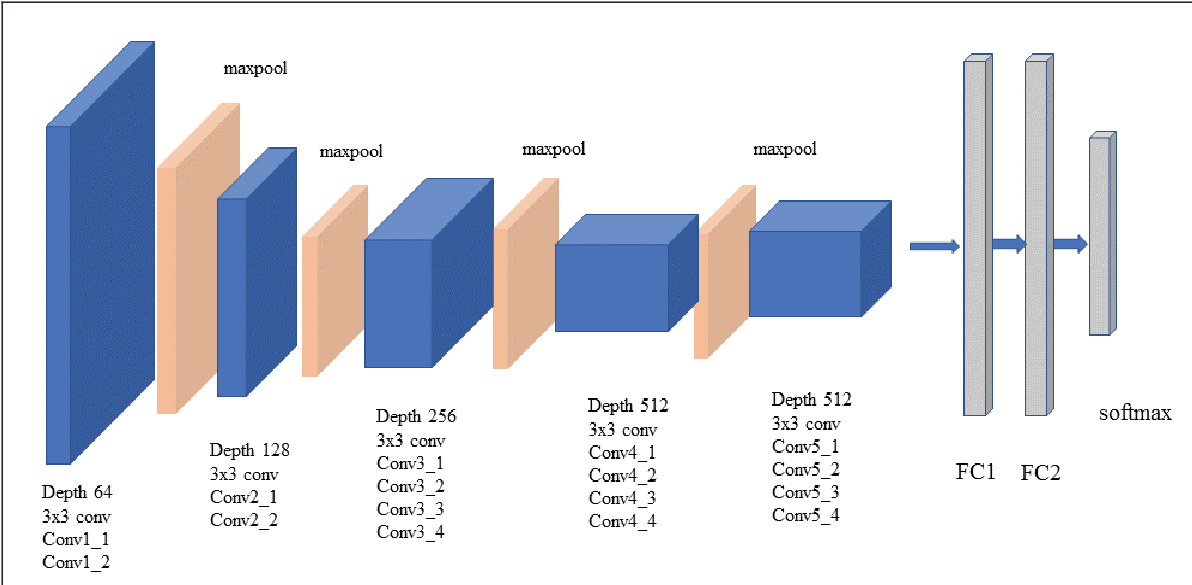
\includegraphics[scale=0.20]{report/Background/images/vgg19.png}
\caption{The VGG-19 network}
\label{fig:rotasjon}
\end{center}
\end{figure}
The VGG-network is responsible for producing the feature space that gives filter responses for the content image and the style image. The filters get more complex with the position of the layer in the network, thus generating a more higher-dimensional representation of the image. Gatys et. al used 16 convolutional and 5 pooling layers of the 19 layer VGG-network. They replaced the max-pooling layers in the network with average-pooling layers since they gave more appealing results. \newline\newline
Let $\vec{p}$ be the content image (the image we want to style), and the $\vec{x}$ be the generated image. Then their feature representations in a layer $l$ can be described by the matrices $P^l$ and $F^l$, where $P^l, F^l\in\mathbb{R}^{N_l\times M_l}$. Here, $N_l$ are the distinct filters in layer $l$, each with feature maps of size $M_l$. 
\subsubsection{Loss functions}
Since one of the goals of the optimization is to make $P^l$ similar to $F^l$, i.e. making the generated image like the original content image, Gatys et. al defined the following loss function, the content loss, between the two feature representations described above:
\begin{equation}
\label{eq:content_loss}
    \mathcal{L}_\text{content}(\vec{p},\vec{x},l)=\frac{1}{2}\sum_{i,j}{(F_{ij}^l-P_{ij}^l)^2},
\end{equation}
where $F_{i,j}$ and $P_{i,j}$ are the activations of the $i$th filter at position $j$ in layer $l$. This loss function is the squared-error loss function. Similarly, they defined the style loss as follows:
\begin{equation}
\label{eq:style_loss}
    \mathcal{L}_\text{style}(\vec{a},\vec{x})=\sum_{l=0}^L{w_lE_l},
\end{equation}
where
\begin{equation}
    E_l=\frac{1}{4N_l^2M_l^2}\sum_{i,j}{(G_{ij}^l-A_{ij}^l)^2}.
\end{equation}
Here $A^l$ is the is the style representation of the style image in layer $l$, and $G^l$ is the style representation of the the generated image. $\vec{a}$ is the style image, and $w_l$ are the weighting factors for how much each layer should contribute to the total loss. $G^l$ is also known as the Gram matrix. This matrix will be discussed in Section \ref{section:gram}. Now, the total loss can be written as:
\begin{equation}
\label{eq:total_loss}
    \mathcal{L}_\text{total}(\vec{p}, \vec{a}, \vec{x})=\alpha\mathcal{L}_\text{content}(\vec{p},\vec{x})+\beta\mathcal{L}_\text{style}(\vec{a},\vec{x})
\end{equation}
Here, $\alpha$ and $\beta$ are weights for the content image and the style image. The higher the weight, the more that loss is minimized, resulting in the stylized image to either be more equal to the content image, or the style image.
\subsubsection{Gram Matrix}
\label{section:gram}
\begin{figure}[!ht]
\begin{center}
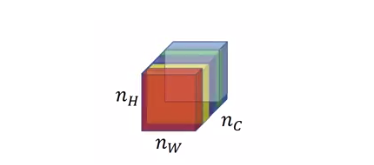
\includegraphics[scale=0.30]{report/Background/images/featuremap.png}
\caption{Feature map with three channels}
\label{fig:featuremap}
\end{center}
\end{figure}
The Gram matrix is a style representation built on top of the CNN. This matrix gives the feature correlations between the vectorised features maps $i$ and $j$ in layer $l$. This correlation is calculated by taking the inner product between the feature maps. Gatys et al. give the following formula for the Gram matrix:
\begin{equation}
    G_{ij}^l=\sum_k{F_{ik}^lF_{jk}^l}
\end{equation}
To understand the Gram matrix, we can reduce the feature maps to 2D vectors. If we have two vectors, say $\vec{a}$ and $\vec{b}$, the closer they are to each other, the more correlated they are. Then the angle between these two vectors will be small, resulting in a large cosine value, giving a large dot product. So the larger the dot product is, the more correlated $\vec{a}$ and $\vec{b}$ are. 
This idea is similar for feature maps. Consider a feature map consisting of three channels, like the one in Figure \ref{fig:featuremap}. The red channel represents the feature of horizontal lines, the yellow represents the feature of vertical lines, and the green represents the features of the color green. If the red channel and the yellow channel have high activation values, then we can say that we have an image of for example a chess board. These two channels will have a higher correlation than that between the yellow channel and the green channel. In a sense, this correlation describes the style of the generated image.
\subsubsection{Gradient descent}
The derivative of the content loss is given by
\begin{equation}
    \frac{\partial\mathcal{L}_\text{content}}{\partial F_{ij}^l}=\begin{cases}
    (F^l-P^l)_{ij}\,&\text{ if }\,F_{ij}^l>0\\
    0\,&\text{ if }\,F_{ij}^l<0.
    \end{cases}
\end{equation}
The derivative of $E_l$ is given by
\begin{equation}
    \frac{\partial E_l}{\partial F_{ij}^l}=\begin{cases}
    \frac{1}{N_l^2M_l^2}\left((F^l)^T(G^l-A^l)\right)_{ji}\,&\text{ if }\,F_{ij}^l>0\\
    0\,&\text{ if }\,F_{ij}^l<0.
    \end{cases}
\end{equation}
The gradients can be calculated by using standard-error back-propagation, as described by Gatys et al.